\chapter{Architecture Design Guidelines}

\section{Observer pattern}

We use our own observer pattern as described in the \w{GoF}. 
Figure \ref{fig:observer-applied} the pattern applies the principle. 
Any object wanting to observe one of the subjects, needs to 
derive from \w{ConcreteObserver}.

\begin{center}
	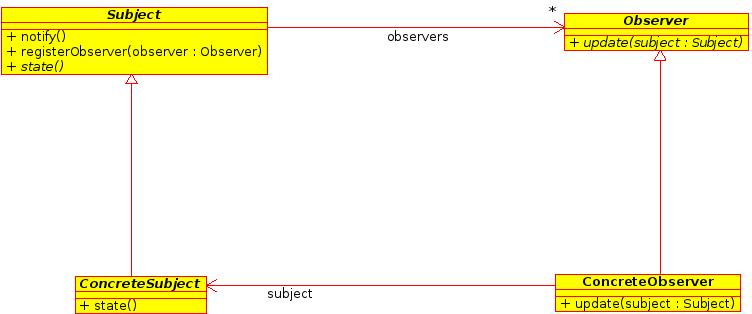
\includegraphics[width=.7\linewidth]{ObserverClassDiagram.jpeg}
	\captionof{figure}{Observer pattern as described in \w{GoF}}
	\label{fig:observer-pattern}
\end{center}

\begin{center}
	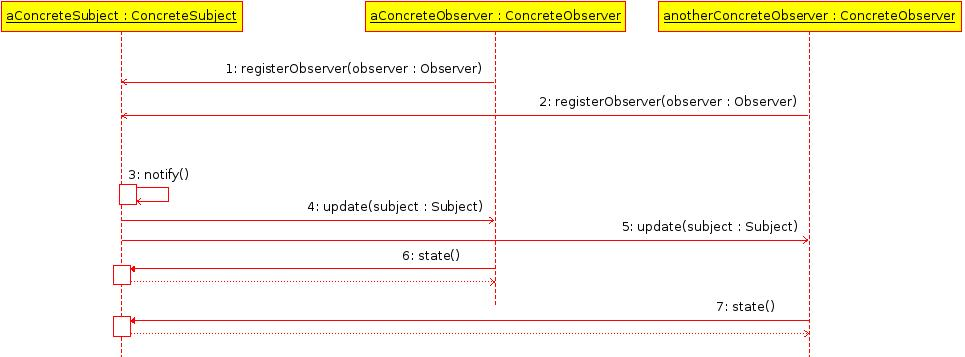
\includegraphics[width=.7\linewidth]{ObserverSequenceDiagram.jpeg}
	\captionof{figure}{Observer pattern applied}
	\label{fig:observer-applied}
\end{center}

\section{Plugin construction}

Any verification tool must override the \w{ConcreteVerificationTool} 
and register with the application in order to have the option
of being executed on request. 

\begin{center}
	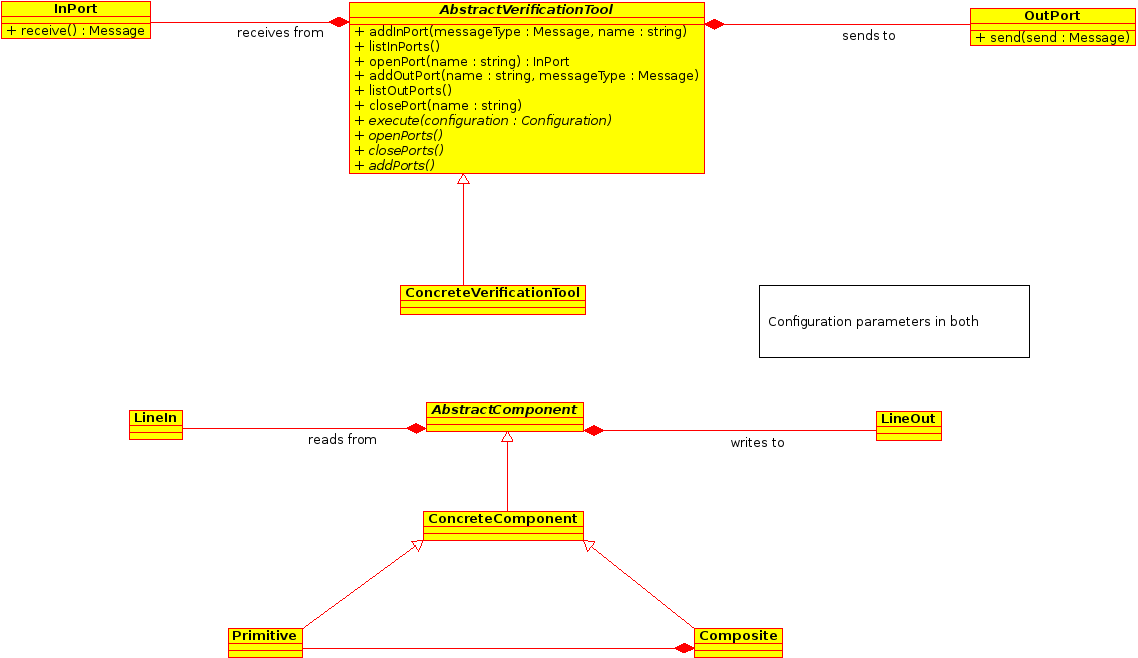
\includegraphics[width=.9\linewidth]{PluginClassDiagram}
	\captionof{figure}{The plugin to build verification tools.}
	\label{fig:plugin-class-diagram}
\end{center}
